\documentclass[12]{article}
\usepackage[spanish,english]{babel}
%\usepackage[spanish]{babel}
\usepackage[utf8]{inputenc}
\usepackage{graphicx}
\usepackage{epsfig}
\usepackage{multirow}
\usepackage{multicol,caption}
\usepackage{amsthm} % Theorem Formatting
\usepackage{amssymb}    % Math symbols such as \mathbb
\usepackage{color}
\usepackage{hyperref}
\usepackage[none]{hyphenat}
\usepackage{appendix}
\renewcommand{\appendixname}{Anexo}
\renewcommand{\appendixtocname}{LISTA DE ANEXOS}
\renewcommand{\appendixpagename}{Anexos}
%\renewcommand{\tablename}{Tabla}
%\def\tablename{Cuadro}% por \def\tablename{Tabla}% 
\newenvironment{Figure}
{\par\medskip\noindent\minipage{\linewidth}}
{\endminipage\par\medskip}
\addto\captionsspanish{%
\def\tablename{Tabla}%
}
\topmargin  = 10pt
\oddsidemargin  = -0.5in
%\headheight = 12pt
%\headsep    = 15pt
%\footskip   = 15pt
\textheight = 21.5 cm
\textwidth  = 18.5cm
\tolerance=10000
\title{\bf{Calculo del factor de perdida de la densidad de flujo de radiación emitida por un diodo led emisor infrarrojo, cuando esta radiación interactúa con la metería; utilizando el modulo motorizado infrarossi y su software de control free infrarossi}}
\author{Julian Salamanca\footnote{jasalamanca@udistrital.edu.co}, Diego Parra\footnote{diegoestudianteud1@gmail.com} \\
  Universidad Distrital, Calle 3 No 26A-40 Bogotá-Colombia\\
  Grupo de Física e Informática ``FISINFOR''
}
\date{\today}
\begin{document}
%\def\tablename{Cuadro}% por \def \tablename{Tabla}% 
\renewcommand{\tablename}{Tabla}
\maketitle
\vspace{-0.8cm}
\selectlanguage{english}
\begin{abstract}
This paper illustrates the calculation of the loss factor flux density of radiation emitted by a LED diode infrared emitter, when this radiation interacts with matter; using construction paper of various colors, the motor module infrarossi  and control software free infrarossi,  in a GNU-Linux environment; highlighting the functionality of this instrument in illustrating the calculation factor in the loss of voltage on the measuring instrument and its proportionality with the flux of radiation emitted by a LED diode emitting infrared radiation when it interacts with matter.\\
{\bf{Keywords:}} Motor module, infrared sensors, microcontroller module bluetooth, electromagnetic wave, reflection, refraction, absorption, attenuation, reflectance, transmittance.
\selectlanguage{spanish}
\begin{center}
{\bf{Resumen}} 
\end{center}
El presente trabajo ilustra el calculo del factor de perdida de la densidad de flujo de radiación emitida por un diodo led emisor infrarrojo, cuando esta radiación interactúa con la metería; utilizando cartulinas de varios colores, el modulo motorizado  infrarossi y su software de control free infrarossi, en un entorno GNU-linux; resaltando la funcionalidad de este instrumento en la ilustración del calculo en el  factor de perdida del voltaje en el instrumento de medida y su proporcionalidad con  la densidad de flujo de radiación emitida por un diodo led emisor infrarrojo, cuando esta radiación interactúa con la metería.
\\
{\bf{Descriptores:}} Modulo motorizado, sensores infrarrojos, microcontrolador, modulo bluetooth, ondas electromagnéticas, reflexión, refracción, absorción, atenuación, reflectancia, transmitancia.
\end{abstract}
%tabla de contenido sin numeracion
%\renewcommand\contentsname{\centering TABLA DE CONTENIDO}
%\thispagestyle{empty}
%\setcounter{page}{1}
%\tableofcontents
%\clearpage
%lista de figuras
%\renewcommand\listfigurename{\centering LISTA DE FIGURAS}
%\listoffigures
%\clearpage
%lista de tablas
% \renewcommand\listtablename{\centering LISTA DE TABLAS}
% \listoftables
% \clearpage
\begin{multicols}{2}
\section{Introducción}
Los fenómenos de las ondas siempre han fascinado nuestros pensamientos y tratamos de acercarnos a estos fenómenos para tratar de entenderlos, es allí donde la física con ayuda de la matemática muestran su majestuosidad, al explicar de manera muy detallada estos fenómenos de transporte; desde el punto de vista clásico en la interacción del flujo de radiación electromagnética con la materia pueden darse varios fenómenos tales como la reflexión, refracción, absorción, atenuación, reflectancia, transmitancia; en estos fenómenos, incide radiación sobre una superficie de muestra y se mide la proporción en la cantidad de radiación que el material absorbe, que deja pasar y la que se refleja, estos cálculos son muy utilizados en espectrofotómetros infrarrojos y en diversos estudios que implican la interacción radiación – materia.   \\\\
En este trabajo se hace un calculo del índice de  reflectancia de las diferentes muestras, enviando radiación infrarroja sobre el material y midiendo el factor de perdida en la intensidad de la radiación electromagnética que incide sobre el detector infrarrojo del vehículo motorizado infrarossi después  que la radiación ha interactuado con la muestra y ha sido reflejada.
\selectlanguage{spanish}
\section{Marco teórico}
Los fotones producidos por el diodo emisor de la fuente emisora de radiación infrarroja se dan debido a que “en los semiconductores, con estructura compleja de las bandas energéticas, son posibles las transiciones indirectas de los electrones de la banda de conducción  a la de valencia acompañadas de la emisión de un fotón. En este caso la recombinación del electrón libre con el hueco se desarrolla con la aparición de un fonón, lo que asegura la conservación del cuasi impulso. Lo más probable es que el fonón sea emitido. Si en el semiconductor se desarrollan procesos de recombinación entre bandas  tanto directa como indirectas, en el espectro de radiación se observan dos bandas de luminiscencia. \\ \\
En la banda prohibida de los semiconductores reales existe una gran cantidad de estados localizados, que están ligados a los átomos de impureza, defectos de la estructura, infracciones de la periodicidad de la estructura en la superficie, etc. Estos estados localizados desempeñan un papel importante  en los procesos de luminiscencia. 
\begin{Figure}	
\center
\begin{tabular}{|l|r|}
\hline
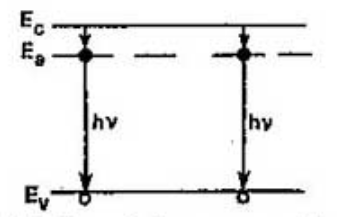
\includegraphics[width=5cm, height=4cm]{img/transiciones.png} \\ \hline
\end{tabular}
\captionof{figure}{Transiciones con radiación entre una banda y los estados de impureza.}
\label{fig:g1}
\end{Figure}
Las transiciones de los electrones de la banda de conducción a los niveles de los pequeños donadores (o de los huecos de la banda de valencia a los niveles de los pequeños aceptores),  que hacen que estos últimos se neutralicen, pueden ser con radiación.. En este caso es de esperar la aparición de luminosidad en la región infrarroja remota del espectro. Pero los cálculos  muestran que en estas transiciones lo más probable es que sea emitido un fonón y no un fotón, es decir, que el proceso se desarrolla sin radiación. La recombinación con radiación se produce por lo general  como viene mostrado en la figura 1. Primero un electrón de la banda de conducción es capturado por un nivel local situado un poco más abajo que Ec  \footnote{Ec es el nivel de energía de conducción.}, y después se efectúa la recombinación de este electrón localizado con un hueco de la banda de valencia, la cual va acompañada de la emisión de un fotón. El electrón puede también realizar una transición con radiación de la banda de conducción y después recombinarse con un hueco. \\
El estudio de los espectros de luminiscencia relacionados a diversas impurezas y defectos permite obtener información sobre estas infracciones de la estructura. \\ \\
Durante la absorción de la luz puede surgir en los semiconductores pares electrón – hueco ligados por la atracción coulombiana, es decir, excitones. Si uno de estos pares se aniquila, se produce la emisión de un fotón. La energía de esta radiación es: 
\begin{equation}
h\nu = E_g - E,
\end{equation}
donde E es la energía de enlace del excitón." \cite{SEMICONDUCTOR} \\ \\
Ahora se tiene un flujo de fotones de energía $h\nu$ saliendo del diodo emisor infrarrojo,  ``como los fotones viajan a la velocidad de la luz deben, de acuerdo con la teoría de la relatividad, tener una masa en reposo igual a cero; de aquí que su energía sea completamente cinética. Si un fotón existe, entonces se mueve a la velocidad de la luz, $c$; si deja de moverse a velocidad c, deja de existir. Para $m_{0} = 0$ la relación relativista momentum – energía  se convierte en $E = pc$.
de esta forma, cada fotón tiene un momentum de 
\begin{equation}
p = \frac{E}{c} = \frac{h\nu}{c} = \frac{h}{\lambda}
\end{equation}
Desde el punto de vista cuántico, un haz de energía electromagnética se compone de fotones que se desplazan a la velocidad $c$. La intensidad del haz será proporcional al número de fotones que cruza un área unitaria por unidad de tiempo. Entonces, si el haz es monocromático (de una frecuencia), la intensidad $I$ se obtendrá de 
\begin{equation}
I = (h\nu)\times \left ( \frac{N}{A\times t } \right)
\end{equation}
$h$ es la constante de Plank que tiene un valor de $6.626 \times 10^{-34} (J * s)$; $N$ es el número de fotones que pasan por segundo a través de la superficie; $A$ es la superficie; $t$ es el tiempo en segundos."\cite{FISICA_MODERNA}\\ \\
Esta radiansa de fotones desde el diodo emisor, avanza por el espacio proyectando un ángulo solido, por lo que la irradiancia  sera igual al cociente de la radiansa con el ángulo solido proyectado.\\\\
La maxima distancia que se toma para la radiansa de fotones es de 27 centimetros desde el diodo emisor hasta el material de muestra \footnote{La muestra son octavos de cartulina de colores.} colocado perpendicular al flujo de energía, por lo que habrá reducido su intensidad con el inverso del cuadrado de la distancia de la fuente a la muestra $\frac{1}{(0.27)^{2}}$ .\\\\
Ahora el flujo de fotones que interactua con la superficie del material de muestra dan como resultado desde el punto de vista clásico varios fenómenos físicos como lo son  la reflexión, refracción, absorción, atenuación, reflectancia, transmitancia.  Ahora el flujo de fotones  es  visto como el flujo de ondas electromagnéticas,   las que interactúan con la materia  en donde parte de la energía es transmitida al material aumentando la energía cinética media de sus constituyentes, otra parte traspasa el material y el resto del flujo electromagnético avanza paralelamente contrario a la dirección de desplazamiento inicial, si no se considera interacción de las ondas electromagnéticas con el aire como medio disipativo  y otras formas de perdida de energía.\\\\
``Consideremos un haz de luz circular que incide en una superficie, tal como se muestra en la figura 2, de tal modo que se produzca una zona iluminada cuya área sea $A$. Recordemos que la potencia por unidad de área que cruza una superficie en el vacío cuya normal es paralela a $\textbf{S}$, el vector de Poynting  viene determinado por:
\begin{equation}
\textbf{S} = c^{2} \epsilon_{0}\textbf{E}\times \textbf{B}
\end{equation}
A demás la densidad de flujo radiante $(W / m^{2})$ o irradiancia es entonces 
\begin{equation}
I =  < S >_{t}   = \frac{c \epsilon_{0}}{2} E_{0}
\end{equation}
Este el promedio de energía por unidad de tiempo que cruza  un área unidad, normal a  $\textbf{S}$ (en medios isótropos $\textbf{S}$ es paralela al vector de onda $\textbf{k})$. En el caso que nos ocupa (figura 2) sean $I_{i} , I_{r}$ y $I_{t}$ las densidades de flujo incidente, reflejado y transmitido, serán respectivamente, $A cos(\theta _{i})$, $A cos(\theta _{r})$ y $A cos(\theta _{t})$.\\ \\
De acuerdo con esto, la potencia incidente es $I_{i} A cos(\theta_{i})$, esta es la energía por unidad de tiempo que fluye en el rayo incidente y, por consiguiente, la potencia que llega a la superficie de $A$. Del mismo modo,  $I_{r} A cos(\theta_{r})$, es la potencia en el rayo reflejado, e $I_{t} A cos(\theta_{t})$, es la potencia que se transmite a través de $A$. Definimos la \textbf{reflectancia} $R$ como el cociente entre la potencia (o flujo) reflejada y la potencia incidente, es decir:
\begin{equation}
R \equiv \frac{I_{r}A cos(\theta_{r})}{I_{i}A cos(\theta_{i})} = \frac{I_{r}}{I_{i}}
\end{equation} 
\begin{Figure}	
\center
\begin{tabular}{|l|r|}
\hline
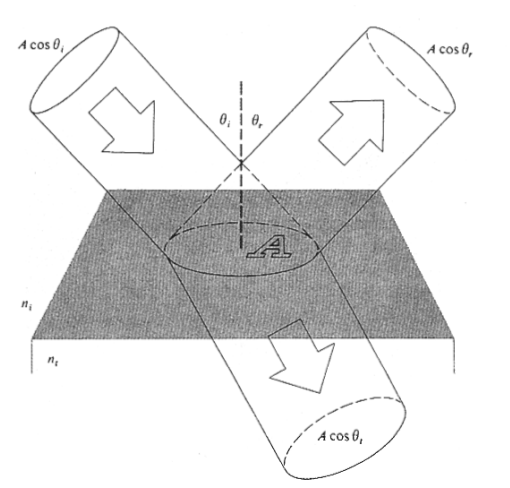
\includegraphics[width=7cm, height=6cm]{img/reflexate.png} \\ \hline
\end{tabular}
\captionof{figure}{Reflexión y transmisión de un haz incidente.}
\label{fig:g2}
\end{Figure}
Del mismo modo la \textbf{transmitancia T} se define como el cociente entre el flujo transmitido y el flujo incidente y viene dada por:
\begin{equation}
T \equiv \frac{I_{t}A cos(\theta_{t})}{I_{i}A cos(\theta_{i})} = \frac{I_{t}}{I_{i}}
\end{equation}
escribamos ahora una ecuación que represente la conservación de energía para la configuración que se muestra en la figura 2. Dicho de otro modo, la energía total que llega al área  $A$ por unidad de tiempo debe ser igual a la energía que fluye hacia fuera de ella por unidad de tiempo:
\begin{equation}
I_{i} A cos(\theta_{i}) = I_{r} A cos(\theta_{r}) + I_{t} A cos(\theta_{t}) 
\end{equation}
multiplicando a ambos lados por $c$ esta expresión queda: 
\begin{center}
$ n_{i} E_{0i}^{2}cos(\theta_{i}) =  n_{i} E_{0r}^{2}cos(\theta_{r}) +  n_{t} E_{0t}^{2}cos(\theta_{t})$
\end{center}
Dividiendo a ambos lados por $ n_{i} E_{0i}^{2}cos(\theta_{i})$ obtenemos:
\begin{equation}
1 = \left ( \frac{E_{0r}}{E_{0i}} \right) ^{2} + \left ( \frac{n_{t}cos(\theta_{t})}{n_{i}cos(\theta_{i})} \right ) \left ( \frac{E_{0t}}{E_{0i}} \right) ^{2}
\end{equation}
Pero esto es simplemente:
\begin{equation}
R + T = 1 
\end{equation}
En donde $n_{i}$ es el índice de refracción del medio del que incide, $n_{t}$ es el índice de refracción en el medio transmitido.”\cite{OPTICA} \\\\
Si tomamos $R$ como la reflectancia y $T$ como el factor de perdida de energía por la muestra, podemos decir que: 
\begin{center}
$I_{fot} = RI_{fot} + TI_{fot} $
\end{center}
En donde $I_{fot}$ , es el flujo de fotones que inciden por unidad de tiempo sobre la superficie, $RI_{fot}$ es el flujo de fotones que son reflejados por unidad de tiempo sobre la superficie y $TI_{fot}$  es el flujo de fotones que se transmitieron sobre la superficie. De esta manera los fotones salen de la muestra con una radiansa de $RI_{fot}$.\\\\
Esta radiansa de fotones desde el punto de vista cuántico $RI_{fot}$, o frente de onda desde el punto de vista clásico $\left ( \frac{E_{0r}}{E_{0i}} \right) ^{2}$, tiene que avanzar ahora 27 centímetros desde la muestra hasta el detector, por lo que ahora disminuirá su intensidad desde la muestra al foto detector con el inverso del cuadrado de la distancia $\frac{RI_{fot}}{(0.27)^{2}}$.\\\\
Al iluminar el diodo receptor infrarrojo con esta energía radiante, ``en el semiconductor por cada fotón absorbido se rompe un enlace y se crea un par electrón-hueco. 
Es importante destacar que no todos los portadores fotogenerados contribuyen a la conducción, ya que una fracción importante de ellos se recombinan antes de llegar al extremo correspondiente del semiconductor. El calculo del incremento de corriente $\Delta I_{e}$, debida al exceso de electrones generados en la banda de conducción, $\Delta n$, es
\begin {equation}
\Delta I_{e} = q\mu _{e}(\Delta n)ES
\end{equation} 
siendo $E$ el campo eléctrico aplicado, $\mu_{e}$ la movilidad de los electrones y $S$ la sección transversal del fotoconductor.\\\\
En condiciones de iluminación, el estado estacionario se alcanza cuando la velocidad de generación de portadores en todo el volumen del semiconductor, $G$, se iguala a la velocidad de recombinación, $R$, es decir $R = G$. para un conductor intrínseco en el cual existe un exceso de portadores, $\Delta n = \Delta p$, la velocidad de recombinación de los portadores vendrá dada por:
\begin{equation}
R = \frac{\Delta n }{\tau} = \frac{\Delta p}{\tau}
\end{equation}
siendo $\tau$ el tiempo de vida media de los portadores fotogenerados. En un semiconductor de longitud $L$ en el que suponemos que el espesor es suficiente para que toda la luz que incide sobre el, sea absorbida en su interior, se tiene ahora para la velocidad de generación de portadores en la banda de conducción:
\begin{equation}
G = \eta n_{fot} = \eta \frac{\frac{P_{i}}{h\nu}}{SL}
\end{equation}
siendo $n_{fot}$ el número de fotones incidentes en el semiconductor por unidad de volumen y de tiempo, y $\eta$ la eficiencia de la conversión en la generación de portadores. El valor $n_{fot}$ se calcula a través del cociente entre la potencia de la luz incidente, $P_{i}$, y la energía de la radiación, $h\nu$, dividido a su vez por el volumen del material.\\ \\
Sabiendo que la velocidad de arrastre de los electrones por el campo eléctrico viene dada por: $v_{e} = \mu_{e}E$, las igualdades anteriores permiten escribir para la corriente de electrones fotogenerada entre los dos electrodos:
\begin{equation}
\Delta I_{e} = q\nu_{e}\eta\frac{\frac{P_{i}}{h\nu}}{L}\tau
\end{equation}
si se tiene en cuenta que el cociente $t_{r} = L/v_{e}$, representa el tiempo de trásito de los electrones entre los dos electrodos, resulta para $\Delta I_{e}$:
\begin{equation}
\Delta I_{e} = q\eta \frac{P_{i}}{h\nu}\frac{\tau}{t_{r}}
\end{equation}
con una expresión similar para la corriente de huecos en la banda de valencia. En la ecuación anterior, el factor $q\eta(P_{i}/h\nu) = I_{fot}$ tiene dimensiones de corriente y representa la velocidad de generación de carga en el semiconductor. En función de este parámetro, se define el factor de ganancia del fotoconductor a través del cociente:
\begin{equation}
\frac{\Delta I}{I_{fot}} = \frac{\tau}{t_{r}}
\end{equation}
ahora bien un diodo operando con cierto voltaje aplicado, $V$, en presencia de radiación electromagnética  capaz de excitar portadores a través de la banda prohibida dejara pasar una intensidad I dada por:
\begin{equation}
I = I_{0}[e^{(qV/kT)}-1] - I_{L}
\end{equation}
donde $I_{0}$ representa la corriente típica de un diodo, $I_{L}$ representa la corriente debida a  los portadores generados. El valor de $I_{L}$ puede calcularse de la siguiente manera:
\begin{equation}
I_{L} = qGS(L_{e} - L_{h})
\end{equation}
siendo $G$ el número de portadores generados por unidad de volumen y de tiempo y $S$ el área de la sección transversal del diodo. $L_{e}$ y $L_{h}$ representan las longitudes de difusión de los electrones y huecos. El dispositivo funciona entonces como detector del nivel de iluminación  convirtiendo una señal óptica en señal eléctrica." \cite{FOTOELECTRICO}\\ \\ 
Como la corriente I en el diodo es proporcional a la irradiancia de la superficie iluminada por fotones infrarrojos y esta ultima se atenúa con el inverso del cuadrado de la distancia del frente de energía a la fuente; en otras palabras como el voltaje que mide el microcontrolador es directamente proporcional a la corriente $I$ en el diodo receptor infrarrojo, por consiguiente el voltaje medido en el semiconductor debe  tener una relación inversamente proporcional al cuadrado de la distancia, para el caso ideal:
\begin{equation}
I_{fot}(x) \propto V(x) = \frac{A_{0}}{x^{2}}
\end{equation}
para este caso en el que el material absorbe  parte de esa energía, solo $RI_{fot} /x^{2}$ estarán incidiendo en la superficie del foto detector infrarrojo por lo que ahora el voltaje medido en el microcontrolador sera:
\begin{equation}
RI_{fot}(x) \propto RV(x) = \frac{RA_{0}}{x^{2}}
\end{equation}
%----------------------aca empieza el montaje experimental-------------------------
\section{Montaje experimental}
\subsection{Materiales del montaje}
Para la realización de este montaje se utilizarón los siguientes materiales:
\begin{enumerate}
\item[a.] Ordenador con sistema operativo GNU-Linux.
\item[b.] Modulo motorizado infrarossi.
\item[c.] Software de control free infrarossi.
\item[d.] Un octavo de cartulina de los siguientes colores: azul, amarilla, roja, verde oscura, negra.
\item[e.] Modulo bluetooth para pc.
\end{enumerate}
\subsection{Montaje}
Situar el vehículo motorizado infrarossi a una distancia de 27 cm de la muestra (octavo de cartulina) tal como se muestra en la figura 3, la muestra debe estar perpendicular a la parte frontal del vehículo. Abrir una terminal de GNU-Linux y escribir infrarossi, oprimir enter y la clave de superusuario, luego de abrir el programa debe oprimir el boton on, esperar que se empareje el bluetooth, una vez emparejado el modulo bluetooth, el programa desplegara un tercer menú, oprimir el botón de absorción y esperar que el programa tome los datos necesarios.\\\\
Ahora el software de control free infrarossi le envía vía bluetooth la señal de avanzar y capturar datos al vehículo motorizado infrarossi el cual avanza 2 milímetros por cada paso, recolecta 140 datos por cada avance enviándolos vía bluetooth al ordenador en donde el software de control realiza un análisis estadístico de los mismos, cuando termina este análisis envía una señal al modulo motorizado infrarossi vía bluetooth, indicándole que avance nuevamente y repita el proceso, esto lo realiza 117 veces; una vez terminado de recoger todos los datos realiza una estadística sobre toda la muestra de estos datos capturados. 
\begin{Figure}	
\center
\begin{tabular}{|l|r|}
\hline \\
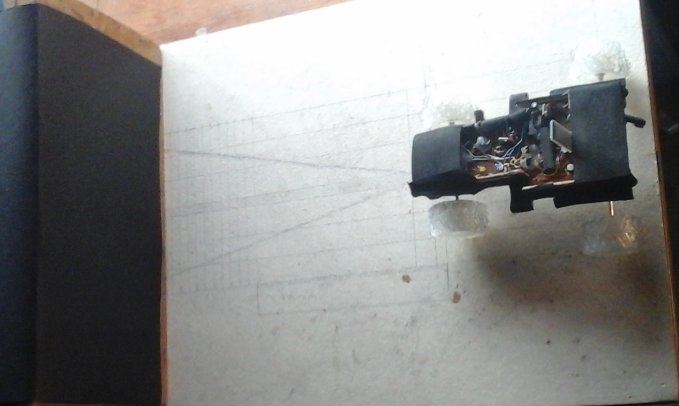
\includegraphics[width=7cm, height=5cm]{img/mon_abso.png} \\\\ \hline
\end{tabular}
\captionof{figure}{Imagen del montaje para la absorción utilizando el modulo motorizado infrarossi y un octavo de cartulina.}
\label{fig:g3}
\end{Figure}
\vspace{0.2cm}
\section{Análisis de resultados}
El programa free infrarossi después de recoger los datos realiza un análisis estadístico de los mismos con un “ajuste lineal de una función exponencial de la forma $Y^{*} = aX^{b}$, siendo $Y$ la variable dependiente, $a$ la amplitud, $X$ la variable independiente,  $b$ el valor del exponente en este caso de atenuación, $Y^{*}$ es el valor esperado de la variable dependiente; aplicando logaritmo natural para linealizar se obtiene:
\begin{equation}
ln ( Y^{*}) = ln (a) + bln(X)  \cdots \Longrightarrow V^{*} = A + bU
\end{equation} 
donde $V^{*}$ es $ln(Y^{*})$, $A $ es el $ln(a)$ y $U$ es igual al $ln(X)$. \\\\
La suma de  todos los errores debe ser diferentes a cero $\sum e \neq 0$. \\\\
El exponente de ajuste b se halla con la varianza de $U$ sobre $V$  dividida entre la varianza de $U$ sobre $U$, obteniendo
\begin{equation}
b = \frac{S_{UV}}{S^{2} _{U}} =  \frac{\frac{1}{n} \sum_{i=1}^{n} UV - \bar{U} \bar{V}}{\frac{1}{n} \sum _{i=1}^{n} U^{2} - \bar{U}^2}
\end{equation}
ahora el valor de A sera igual al valor medio del logaritmo de la variable dependiente $\bar{V}$ menos el valor de la multiplicación entre el exponente $b$ y el valor medio del logaritmo de la variable independiente:
\begin{equation}
A = \bar{V} -b\bar{U}
\end{equation}
deshaciendo el logaritmo de $A$  se obtiene el valor de la amplitud a:
\begin{equation}
a = antiln(A) = antiln(\bar{V} – b\bar{U})
\end{equation}
de modo que el ajuste efectuado es:
\begin{equation}
Y^{*} =  aX^{b}  = [antiln(\bar{V} - b\bar{U})]*X^{ \left(\frac{\frac{1}{n} \sum_{i=1}^{n} UV - \bar{U} \bar{V}}{\frac{1}{n} \sum _{i=1}^{n} U^{2} - \bar{U}^{2}}\right)}
\end{equation}
la bondad del ajuste es el error cuadrático medio o $ECM$ y es igual a: 
\begin{equation}
ECM = \frac{\sum_{i=1}^{n}e_{i}^{2}}{n}
\end{equation}
siendo $e_{i}$ cada una de las diferencias entre las variables dependientes y los valores estimados para las variables dependientes $e_{i} = Y_{i} - Y^{*}_{i}$; al haber transformado la variable dependiente ya no se minimiza $\sum e^{2}$ sino $\sum (ln(Y) – ln(Y^{*}))^{2}$, de ahí que $\sum e \neq 0$."\cite{ESTADISTICA}\\\\
Este análisis se realizo previamente con un espejo, el cual deja como patrón de referencia o de voltaje ideal, el  valor medio de $0.0277 X ^{-2}$  y en la figura 4 aparece con el nombre $V_{1}$; ahora el programa calcula un valor estimado para los datos de la siguiente manera: el voltaje perdido $V_{p}$ debe ser igual al voltaje ideal $V_{1}$ menos el voltaje que mide el microcontrolador osea el voltaje real $V_{real}$ .
\begin{center}
$V_{p} = V_{1} - V_{real}$
\end {center}
El factor de perdida en el voltaje $T$ debe ser igual al cociente del voltaje perdido $V_{p}$ y el voltaje ideal $V_{1}$
\begin{center}
$T=\frac{V_{p}}{V_{1}} $
\end{center}
por lo tanto el promedio en el factor de perdida debe ser igual a la transmitancia o mejor dicho a la energía que se transmitió a la muestra,  
\begin{center}
$\bar{T} = \sum{T_{i}}/N$
\end{center} 
como la reflectancia es igual a $R = 1 – T $ (ecuación 10), el valor de la amplitud $a$, debe ser igual:
\begin{center}
 $ a = (1 – \bar{T}) (0.0277)$
\end{center}
por lo que ahora el voltaje estimado $V2^{*}$ en función del inverso de la distancia, disminuye con la reflectancia $R$: 
\begin{center}
 $ V2^{*} = (1 – \bar{T}) (0.0277) X^{-2}$
\end{center}
después de este análisis el software free infrarossi  realiza la gráfica mostrando en ella (figura 4) el voltaje ideal $V1(x)$, el voltaje estimado debido a la reflectancia $V2^{*}$ y el factor de transmitancia o factor de perdida en el voltaje $F_{p}$.
\vspace{0.3cm}
\begin{Figure}	
\center
\begin{tabular}{|l|r|}
\hline
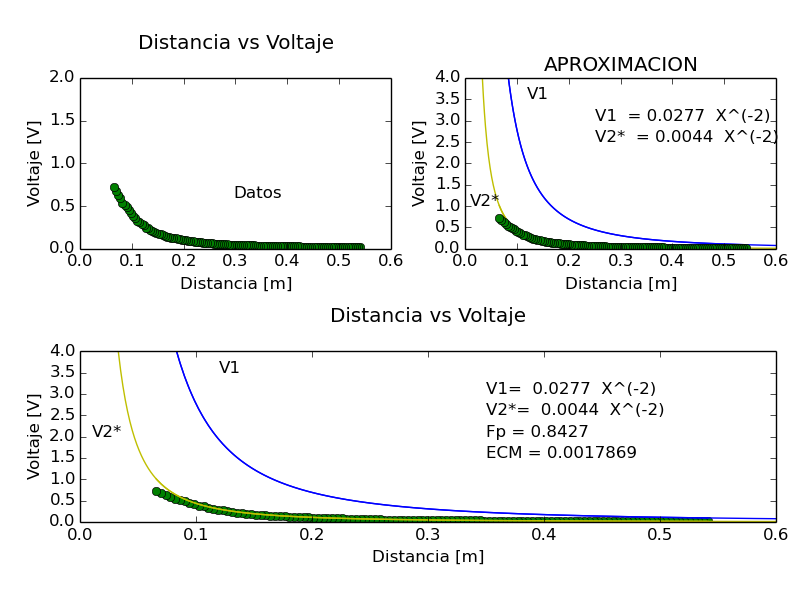
\includegraphics[width=8cm, height=6cm]{img/azul.png} \\ \hline
\end{tabular}
\captionof{figure}{Imagen generada por el programa free infrarossi, donde se aprecia los datos capturados en el experimento, las funciones de color azul en la gráfica es el voltaje ideal $V1$, la función de color amarillo es la gráfica estimada $V2^{*}$ y los puntos de color negro son los datos recolectados. }
\label{fig:g4}
\end{Figure}
En la tabla 1 se muestra  la densidad de voltaje $\bf{a}$ en $V/m^{2}$ , estimado por el software free infrarossi, para cada una de las diferentes muestras del mismo material de cartulina pero diferentes pigmentos; la cartulina en la cual hubo más transmitancia fue la de color negro, pues el $86.72\%$ de intensidad de la luz incidente sobre ella fue transmitida al material, llegando solo un $13.28\%$ de esta al sensor; ahora la muestra que mayor reflectancia tubo fue la de color rojo pues el $18.17\%$ de la intensidad lumínica llego al sensor, indicando que solo el $81.83\%$ de esta fue transmitida al material de muestra.
\begin{center}
\begin{tabular}{|l|c|c|c|c|} 
\hline
\bf{Color} & \textbf{a} & \bf{T} & \bf{R} & \textbf{ECM}\\
\hline
 Azul & 0.0044 & 0.8427 & 0.1573 & 0.001786\\
\hline
 Amarillo & 0.0043 & 0.8436  & 0.1564 & 0.002051\\
\hline
 Verde & 0.0047 & 0.8299  & 0.1701 & 0.002794\\
\hline 
 Negro & 0.0037 & 0.8672  & 0.1328 & 0.000295\\
\hline
Rojo & 0.005 & 0.8183  & 0.1817 & 0.000389\\
\hline
\hline
\end{tabular}
\\
\end{center}
\textbf{Tabla 1.} Datos  de amplitud, transmitancia y reflectancia de cinco muestras de cartulina de diferentes colores, recolectados con el modulo motorizado infrarossi y su software de control free infrarossi.\\ \\ 
El error cuadrático medio indica que el valor estimado para la densidad de voltaje que se produce en el diodo cuando sobre este incide radiación infrarroja que ha interactuado con la muestra, es explicado en un $99.97\%$ con este tratamiento (figura 5 y 6).  
\begin{Figure}	
\center
\begin{tabular}{|l|r|}
\hline
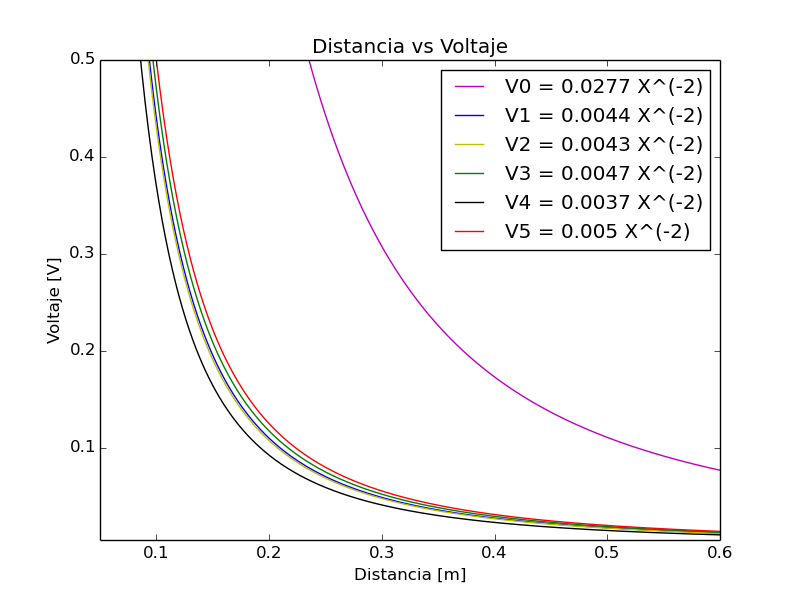
\includegraphics[width=8cm, height=6cm]{img/reflectancia.png} \\ \hline
\end{tabular}
\captionof{figure}{Imagen generada con la librería matplotlib de python 2.7, donde se aprecia las funciones estimadas por el programa y la función ideal de densidad de voltaje. }
\label{fig:g5}
\end{Figure}
\begin{Figure}	
\center
\begin{tabular}{|l|r|}
\hline
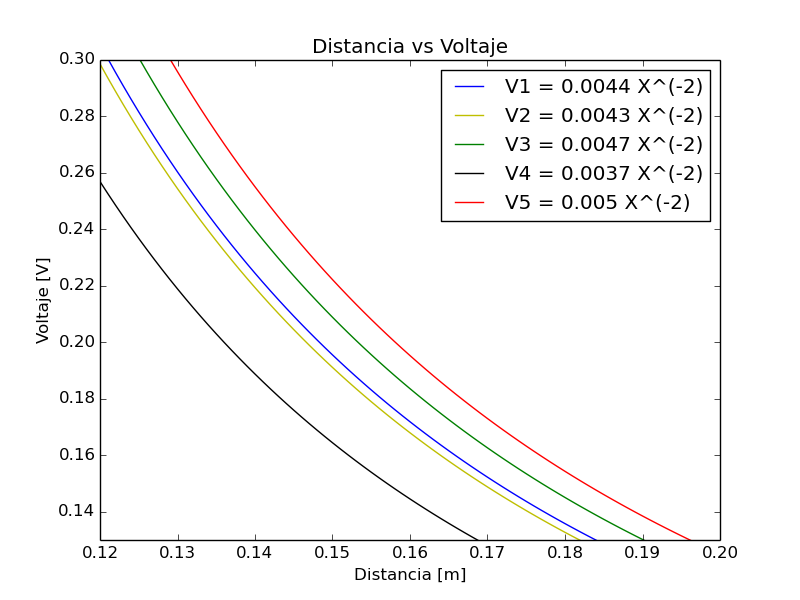
\includegraphics[width=8cm, height=6cm]{img/reflectancia2.png} \\ \hline
\end{tabular}
\captionof{figure}{Imagen generada con la librería matplotlib de python 2.7, donde se aprecia una porción distinguible de las funciones estimadas por el programa.}
\label{fig:g6}
\end{Figure}
\section{Conclusiones}
\begin{enumerate}
\item[*]  La muestra en la cual hubo más transmitancia, es la cartulina de color negro, pues el $86.72\%$ de intensidad de la luz incidente sobre ella fue transmitida al material, llegando solo un $13.28\%$ de esta al sensor.
\item[*]  La muestra que mayor reflectancia tubo fue la de color rojo pues el $18.17\%$ de la intensidad lumínica llego al sensor, indicando que solo el $81.83\%$ de esta fue transmitida al material de muestra.
\item[*] El modulo motorizado infrarossi y su software de control ilustran de manera cuantitativa y cualitativa fenómenos ondulatorios y corpusculares  de la radiación electromagnética como la atenuación con el inverso del cuadrado de la distancia, la radiansa, la irradiancia, fenómenos de transporte e  inyección, calculando el factor de perdida de voltaje en el sensor y de esta manera predice los valores de reflectancia y transmitancia del material estudiado.  
\item[*] El error cuadrático medio indica que solo el $0.03\%$ del experimento no se explica con este modelo físico–matemático, dejando un $99.97\%$ de fiabilidad en el ajuste estadístico utilizado en este trabajo.
\item[*] La física que se encuentra de manera implícita y explicita en este trabajo hace que el instrumento motorizado infrarossi y su software de control free infrarossi sea un herramienta indispensable  en el aula de clase,  tanto de profesionales como estudiantes de ciencias afines.
\end{enumerate}
% ---------------------Aca empieza la bibliografia----------------------------------------------
\begin{thebibliography}{99}
\bibitem{SEMICONDUCTOR} Shalímova, K. V., \& Grdiam, A. (1975). Física de los Semiconductores.
\bibitem{FISICA_MODERNA} Gautreau, R., Savin, W., \& Velazquez Valle, D. R. (2001). Fisica moderna.
\bibitem{OPTICA} Hecht, E., Dal Col, R., Talavera, R. W., \& Pérez, J. M. G. (2000). Óptica. Addison Wesley.
\bibitem{FOTOELECTRICO} Albella, J. M., \& Martínez-Duart, J. M. (1996). Fundamentos de electrónica física y microelectrónica. Addison-Wesley Iberoamericana.
\bibitem{ESTADISTICA} Ostle, B. (1981). Estadística aplicada. Limusa.
\bibitem{FISICA4} Miákishev, G. (1995). Bujovsev. Física 4. Editorial Mir Moscú. Moscú. 
\bibitem{ESTADO_SOLIDO} Pavlov, P. V., \& Jojlov, A. F. (1987). Física del estado sólido. Rubiños-1860.
\bibitem{PYTHON} Gift, N., \& Jones, J. M. (2008). Python for Unix and Linux system administration. ``O'Reilly Media, Inc.".
\bibitem{BASH} Álamos Zorrilla, J. (2004). Programación orientada a objetos con shell-bash. SÓLO PROGRAMADORES LINUX.
\bibitem{COMPUTO} David P. Sanders (2013). Notas del curso para el computo científico. Curso de actualización académica de la DGAPA-UNAM..
\end{thebibliography}
\end{multicols}
\end{document}

